%% Incluindo os pacotes necessários 
\documentclass[12pt, a4paper]{article}
\usepackage[utf8]{inputenc}
\usepackage[portuguese]{babel}
\usepackage{titlesec}
\usepackage{titling}
\usepackage{enumitem}
\usepackage{indentfirst}
\usepackage{graphicx}
\graphicspath{{images/}}
\usepackage{fancyhdr}
\usepackage{color}
\usepackage{fancyhdr}
\usepackage{colortbl}
\usepackage{framed}

%% Definindo o Autor e o título
\author{Gustavo Juliano Borges \and Victor Emanuel Almeida \and Marco Aurélio Guerra Pedroso}
\title{Documentação do Projeto I~-~IES}

%% Estilo da página
\pagestyle{fancy}
\fancyhead[L]{Documentação~-~Projeto I}
\fancyhead[R]{Introdução Engenharia de Software}
\fancyfoot[L]{Outubro~-~2020}
\fancyfoot[C]{}
\fancyfoot[R]{-~\thepage~-}
\renewcommand{\headrulewidth}{0.7pt}
\renewcommand{\footrulewidth}{0.3pt}

%% Definindo espaçamento
\titlespacing{\section}{0pt}{*2}{*1.1}
%%\titlespacing{\subsection}{}{}{}

\titleformat{\section}
{\Large\bfseries}
{\thesection}
{.5cm}
{}

\pretitle{\vfill\begin{center}\LARGE}
\postdate{\end{center}\vfill}

\begin{document}
\begin{titlepage}
\maketitle\thispagestyle{empty}
\end{titlepage}
\section{Introdução}

Foi proposto pelo professor a elaboração de um programa que simula um streaming de vídeo.

Sendo assim criamos uma equipe formada por~\textbf{\theauthor}, e nomeamos nosso software de \textbf{Data Streaming Video System} \textbf{(DSVS)}

\section{Casos de uso}

\subsection{Cadastrar um vídeo}
Caso de Uso no qual o usuário final cadastra um novo vídeo a base de dados de vídeos.
\begin{enumerate}
	\item Entrar no menu Principal do DSVS
	\item Entrar no Menu de vídeos
	\item Entrar no menu de adicionar vídeos
	\item Entrar com os dados do vídeo
		\begin{enumerate}
			\item Entrar com o tipo de vídeo
			\item Entrar com o nome do vídeo
			\item Entrar com o nome do diretor
			\item Entrar com a duração do vídeo
				\begin{itemize}
					\item quantidade total de horas
					\item quantidade total de minutos
					\item quantidade total de segundos
				\end{itemize}
			\item Entrar com o número de temporadas
			\item Entrar com o número de gêneros
			\item Entrar com os gêneros
		\end{enumerate}
	\item Voltar ao menu de vídeos
	\item Voltar ao menu principal
	\item Encerrar o programa
\end{enumerate}
\subsection{Cadastrar um novo usuário}
	Caso de Uso, no qual ocorre um erro no qual o usuário, já existente ou novo, cadastra-se.
\begin{enumerate}
	\item Entrar no Menu de usuário
	\item Entrar no Menu de adicionar usuário
	\item Entrar com os dados do usuário
		\begin{enumerate}
			\item Entrar com o nome
			\item Entrar com a data de nascimento (Ano $>$ Ano-Atual)
			\item FALHA
		\end{enumerate}
	\item Mensagem de falha
	\item Encerrar programa
	
\end{enumerate}

\section{Diagrama UML}
\begin{figure}[!htb]
	\centering
	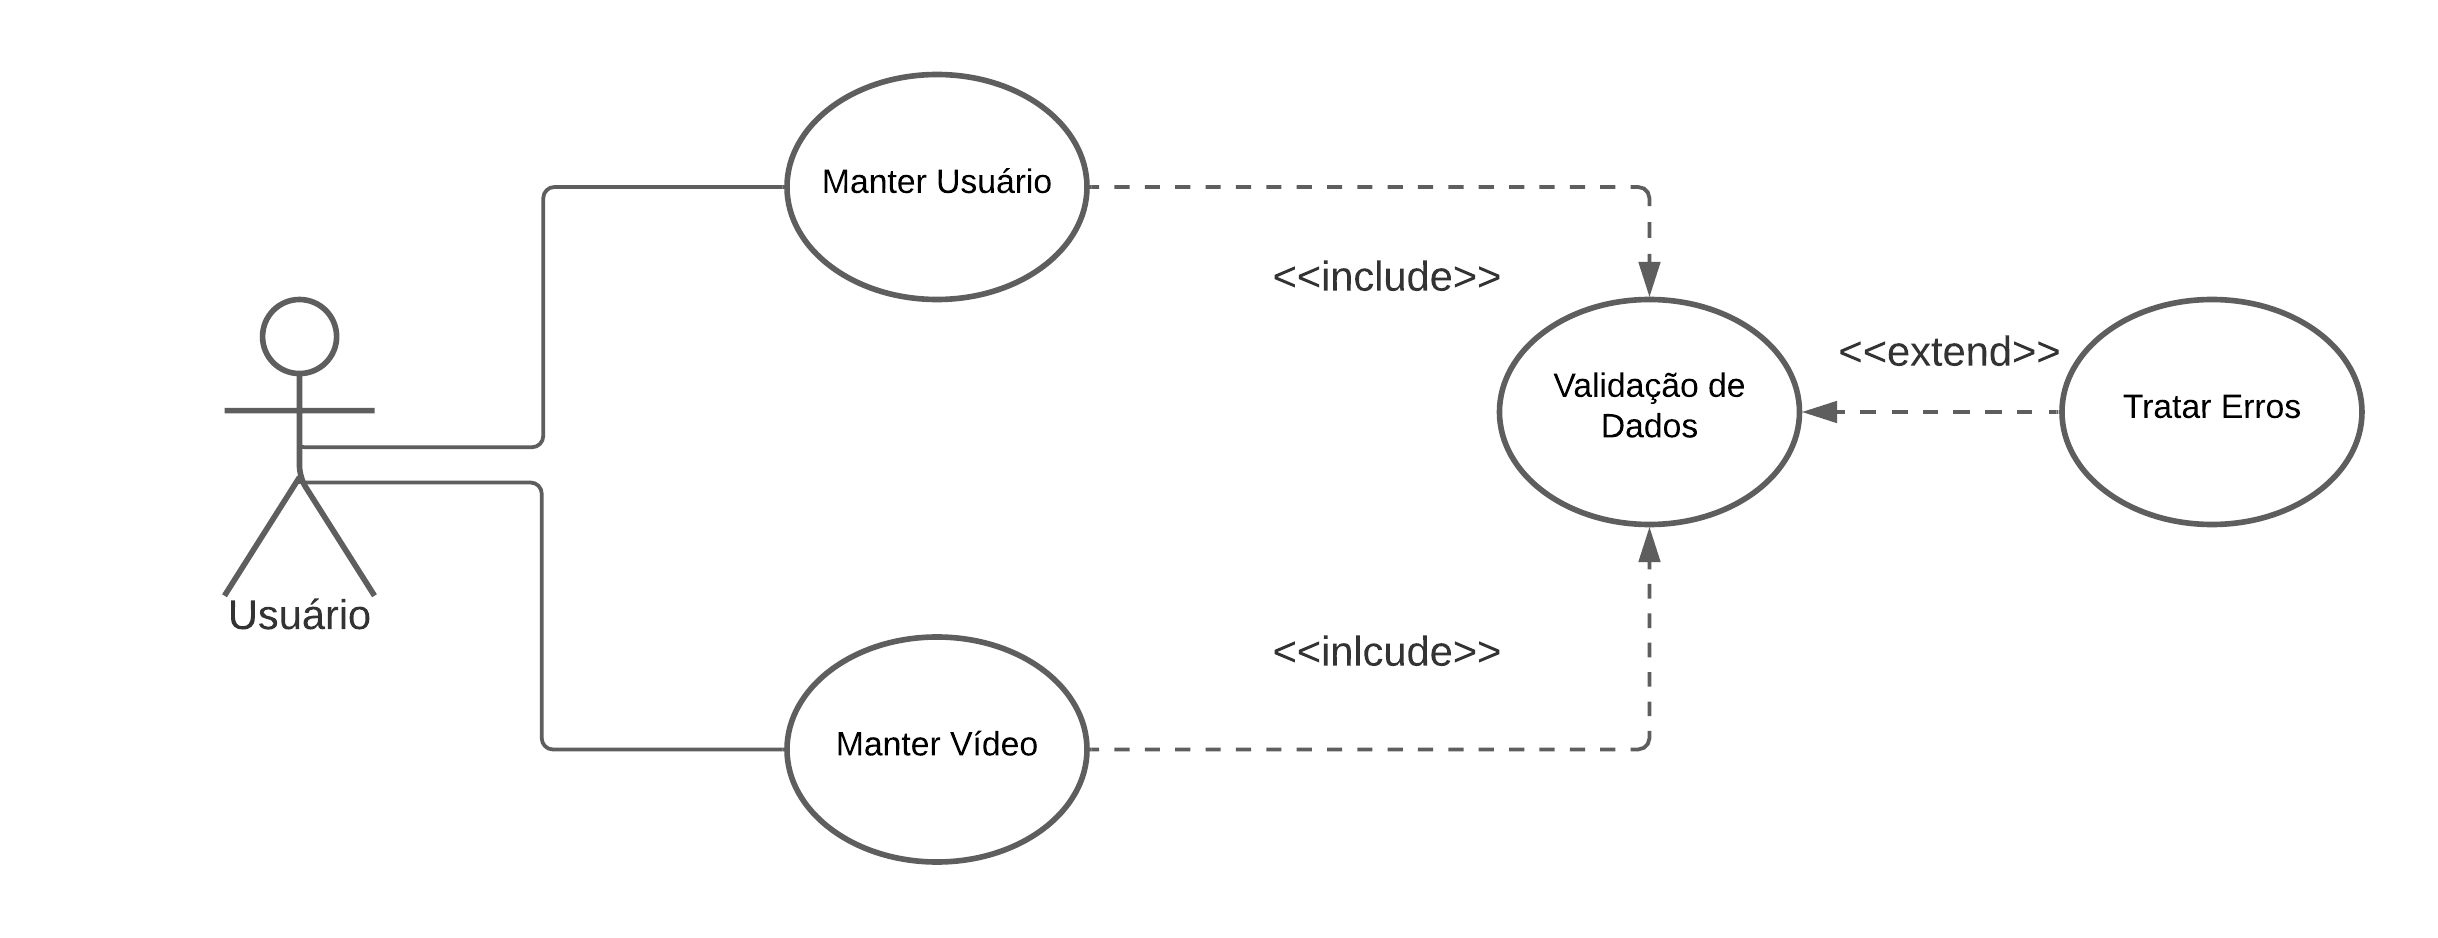
\includegraphics[keepaspectratio, width=\textwidth]{DiagramaUML.png}
	\caption{\label{fig:DiagramaUML.png} Diagrama UML de casos de uso para sistema de streaming}
\end{figure}

\pagebreak
\section{Instruções para o uso do software}

Quando o usuário final executa o código ele se depara com uma mensagem inicial, dando-o boas vindas e o informando quais teclas são utilizadas para se mover entre os menus, sendo elas (w) $ \uparrow $ e a tecla (s) $ \downarrow $.

Tendo selecionado a opção desejada basta apertar ENTER e dessa maneira o programa realizará a ação. Como podemos ver na Figura abaixo:
%\begin{figure}[!htb]
	%\centering
	%\includegraphics[keepaspectratio]{}
	%\caption{\label{fig:}}
%\end{figure}

%Falar da forma de se locomover (W, S)

\subsection{Menu Principal}
Logo após entra-se no Menu principal do programa, que disponibiliza entrar em outros dois menus, sendo o primeiro menu para realizar operações nos dados de usuários e o outro menu para realizar operações nos dados de vídeo.
\begin{figure}[!htb]
	\centering
	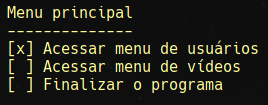
\includegraphics[keepaspectratio]{MenuPrincipal.png}
	\caption{\label{fig:MenuPrincipal.png}Print do Menu Principal}
\end{figure}
\subsection{Menu de Usuários}
Caso dentro do Menu Principal o usuário escolha a opção ``Acessar menu de usuários'', ele se deparará com uma tela assim.

\begin{figure}[!htb]
	\centering
	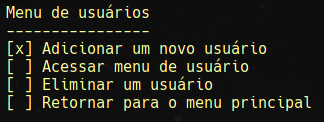
\includegraphics[keepaspectratio]{MenuPUsuarios.png}
	\caption{\label{fig:MenuPUsuarios.png}Print do Menu de Usuários}
\end{figure}
No qual ele poderá realizar as ações de:
\begin{itemize}
	\item Cadastrar um novo usuário: no qual será pedido todas as informações deste usuário, o qual serão entradas via teclado.
	\item Eliminar um usuário: Sendo informado um nome, o programa removerá este usuário.
	\item Menu de usuário: Caso seja escolhida essa opção o programa pede um nome de usuário válido, e entra em um novo menu no qual pode-se:
		\begin{itemize}
			\item Imprimir as informações deste usuário.
			\item Mudar qualquer informação, deste usuário, uma a uma ou todas de uma vez.
		\end{itemize}

\end{itemize}
\subsection{Menu de Vídeos}
Caso dentro do Menu Principal o usuário escolha a opção “Acessar menu de vídeos”, ele se deparará com uma tela assim.

\begin{figure}[!htb]
	\centering
	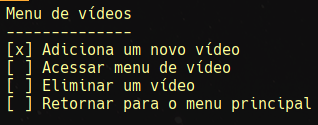
\includegraphics[keepaspectratio]{MenuVideo.png}
	\caption{\label{fig:MenuVideo.png} Print do Menu de Vídeos}
\end{figure}
No qual ele poderá realizar as ações de:
\begin{itemize}
	\item Cadastrar um novo vídeo: no qual será pedido todas as informações deste vídeo, o qual serão entradas via teclado.
	\item Eliminar um vídeo: Sendo informado um nome, o programa removerá este vídeo.
	\item Menu de vídeo: Caso seja escolhida essa opção o programa pede um nome de vídeo válido, e entra em um novo menu no qual pode-se:
		\begin{itemize}
			\item Imprimir as informações deste vídeo.
			\item Mudar qualquer informação, deste vídeo, uma a uma ou todas de uma vez.
		\end{itemize}
\end{itemize}

\clearpage
\subsection{Finalizar o processo}

Tendo realizado todas as operações desejadas o usuário deverá voltar para o Menu Principal, selecionado a opção ``Retornar ao menu principal'':

\begin{figure}[!htb]
	\centering
	
\includegraphics[keepaspectratio]{Retornar.png}
	\caption{\label{fig:Retornar.png} chama o retorno ao Menu Principal}
\end{figure}

Chegando ao Menu principal deve-se selecionar a opção ``Finalizar Programa''. 

\begin{figure}[!htb]
	\centering
	
\includegraphics[keepaspectratio]{finalizar.png}
	\caption{\label{fig:finalizar.png} Encerra o Menu Principal}
\end{figure}

Sendo encerrada a função do Menu Principal, o Programa realiza a escrita no arquivo de todas as estruturas válidas, tanto de vídeo como de usuário.

Ao mesmo Tempo em que o programa realiza ações ele escreve o que esta fazendo no log, que esta localizado na pasta logs na raiz do projeto.
\end{document}
